\section{Zum Mensch-Maschinen-Verhältnis: Kleine Geschichte der KI}

\subsection{Einführung: Technikentwicklung und Mensch-Maschinen-Verhältnis}

Die Vorlesung untersucht das Verhältnis von Mensch und Maschine
am Beispiel der Geschichte der Künstlichen Intelligenz.

Im Zentrum steht dabei nicht nur die technische Entwicklung von KI,
sondern auch die Frage,
welche Vorstellungen vom Menschen
in technischen Systemen und Erklärungen von Technikentwicklung enthalten sind.

Die Geschichte der KI ist daher nicht nur eine Geschichte
von Computern,
Programmen und Algorithmen.

Sie ist zugleich eine Geschichte darüber,
wie Menschen ihre eigenen Fähigkeiten,
Grenzen und Fehler im Vergleich zu Maschinen verstehen.

Zentrale Leitfragen:

\begin{itemize}
\item Warum entwickeln Menschen Technik?
\item Welche Vorstellungen vom Menschen liegen Technikentwicklung zugrunde?
\item Weshalb erscheinen Maschinen oft als überlegen?
\item Welche Rolle spielt menschliche Fehlbarkeit in der Technikgeschichte?
\item Was verändert KI am Verhältnis von Mensch und Maschine?
\end{itemize}

Die Vorlesung zeigt,
dass Technikentwicklung immer auch mit Hoffnungen,
Ängsten,
Machtvorstellungen und Menschenbildern verbunden ist.

\subsection{Effekte der Technikentwicklung seit 1800}

Seit etwa 1800 veränderte Technik
die Lebensbedingungen grosser Teile der Bevölkerung grundlegend.

Technische Entwicklung führte zu höherer Produktivität,
neuen Produktionsweisen
und wachsendem Wohlstand für viele Menschen.

Sie trug dazu bei,
den Lebensstandard zu erhöhen
und die Abhängigkeit von unmittelbarer Subsistenzwirtschaft zu verringern.

Lebensmittelproduktion,
Mobilität,
Kommunikation,
Bildung und Arbeit wurden zunehmend technisch organisiert.

Wichtige Effekte waren:

\begin{itemize}
\item höhere Produktivität
\item mehr Wohlstand für grosse Teile der Bevölkerung
\item Erhöhung des Lebensstandards
\item Überproduktion von Lebensmitteln
\item Alphabetisierung und Bildung
\item neue Formen politischer und gesellschaftlicher Teilhabe
\end{itemize}

Gleichzeitig veränderte Technik auch die Lebensweise
und Arbeitsweise der Menschen.

Der Alltag wurde neu strukturiert.

Die Trennung von Arbeiten und Wohnen,
die Entstehung der Fabrik,
neue Tagesabläufe
und neue Formen von Lohnarbeit
prägten moderne Gesellschaften.

\subsection{Technik, Gesellschaft und neue Organisationsformen}

Technikentwicklung seit 1800 führte nicht nur
zu neuen Maschinen,
sondern auch zu neuen Organisationsformen.

Fabriken,
Fabrikordnungen,
Fliessbandarbeit,
Management,
Spezialisierung
und Informationsverarbeitung
veränderten die Art,
wie Menschen arbeiteten und zusammenlebten.

Dabei entstanden auch neue gesellschaftliche Figuren.

Dazu gehörten:

\begin{itemize}
\item Unternehmer
\item Fabrikarbeiter und Proletariat
\item Fabrikanten
\item Angestellte
\item Manager
\end{itemize}

Zugleich entstanden neue politische Ideologien
und gesellschaftliche Bewegungen.

Sozialismus,
Marxismus,
Kapitalismus,
Liberalismus,
Sozialdemokratie,
Frauenrechtsbewegung
und Faschismus
sind auch im Zusammenhang
mit den Umbrüchen technischer und industrieller Moderne zu verstehen.

Technik erzeugte daher nicht nur materielle Veränderungen,
sondern auch Erwartungen,
Hoffnungen und Ängste.

\subsection{Machbarkeitsfantasien und gesellschaftliche Gestaltung}

Ein zentrales Merkmal moderner Technikentwicklung
ist die Vorstellung,
dass nicht nur Produktionsprozesse,
sondern auch Gesellschaften
technisch geplant,
modelliert und gestaltet werden könnten.

Technik erzeugt dadurch Machbarkeitsfantasien.

Wenn Maschinen,
Fabriken und Infrastrukturen planbar erscheinen,
liegt die Vorstellung nahe,
auch soziale Ordnung,
Arbeit,
Bildung,
Gesundheit
oder Verhalten gezielt gestalten zu können.

Wissenschaft und Technik liefern dabei
eine scheinbar rationale Legitimation.

Gezielte Eingriffe in Gesellschaftsentwicklung
erscheinen dadurch nicht nur möglich,
sondern oft auch notwendig.

Die zentrale Frage lautet daher:

Was treibt Technikentwicklung eigentlich an?

\subsection{Technik als Problemlösung}

Ein erstes Erklärungsmodell versteht Technik
als Antwort auf menschliche Probleme und Bedürfnisse.

Technik entsteht demnach,
weil Menschen bestimmte Herausforderungen bewältigen wollen.

Dazu gehören etwa:

\begin{itemize}
\item Energiebedarf
\item Mobilität
\item Kommunikation
\item Produktion
\item Informationsverarbeitung
\end{itemize}

Nach diesem Modell lösen technische Innovationen
konkrete Probleme.

Seit 1800 entstanden zudem Pfadabhängigkeiten.

Das bedeutet,
dass einmal eingeführte technische Lösungen
weitere technische Entwicklungen nach sich ziehen.

Wenn ein Bereich technisch organisiert wird,
entstehen neue Bedürfnisse,
neue Standards
und neue Folgeprobleme,
die wiederum technisch gelöst werden sollen.

Dieses Modell erklärt jedoch nicht vollständig,
weshalb sich bestimmte Lösungen durchsetzen
und andere nicht.

\subsection{Technik als Wachstumsmotor}

Ein zweites Erklärungsmodell betont
wirtschaftliche Interessen.

Technikentwicklung wird hier durch Wettbewerb,
Profit und Effizienz vorangetrieben.

Unternehmen entwickeln Technik,
um Kosten zu senken,
Produktivität zu steigern
und Märkte zu erweitern.

Technik erscheint damit als Motor
kapitalistischen Wachstums.

Maschinen,
Automatisierung
und digitale Systeme
werden eingesetzt,
um Arbeitsprozesse effizienter zu machen
und wirtschaftliche Vorteile zu erzielen.

Dieses Modell erklärt besonders gut,
weshalb Technik häufig dort entsteht,
wo sie ökonomisch verwertbar ist.

Es zeigt aber weniger,
warum bestimmte technische Vorstellungen
kulturell oder politisch attraktiv werden.

\subsection{Wissenschaft, Fortschrittsglaube und technische Dynamik}

Ein weiteres Erklärungsmodell betont
die Rolle von Wissenschaft und Fortschrittsglauben.

Neue wissenschaftliche Erkenntnisse
führen demnach zu technischen Innovationen.

Technischer Fortschritt erscheint dadurch
als Folge wissenschaftlicher Erkenntnis
und als Ausdruck rationaler Notwendigkeit.

Dieses Modell ist besonders eng verbunden
mit dem modernen Glauben an Wissenschaft,
Objektivität und Fortschritt.

Gleichzeitig stellt sich die Frage,
ob Technik nicht auch eigene Dynamiken entwickelt,
die sich teilweise von wissenschaftlichen Zielen lösen.

Technische Systeme können weiterentwickelt werden,
weil sie bereits existieren,
weil sie wirtschaftlich genutzt werden
oder weil sie neue Probleme erzeugen,
die wiederum technische Lösungen verlangen.

\subsection{Staat, Militär und Krieg}

Ein weiteres wichtiges Erklärungsmodell
betont die Rolle von Staat,
Militär und Krieg.

Viele Technologien wurden durch staatliche Förderung
oder kriegerische Auseinandersetzungen beschleunigt.

Dies gilt besonders für:

\begin{itemize}
\item Computertechnik
\item Raketentechnik
\item Kommunikationstechnologien
\item Überwachungssysteme
\item militärische Automatisierung
\end{itemize}

Technologien,
die zunächst für militärische Zwecke entwickelt wurden,
diffundierten später häufig in zivile Bereiche.

Dadurch zeigt sich,
dass Technikentwicklung nicht nur
aus individuellen Bedürfnissen
oder wirtschaftlichem Wettbewerb entsteht,
sondern auch aus politischen
und militärischen Machtinteressen.

\subsection{Soziale Konstruktion von Technik}

Ein weiteres Modell argumentiert gegen Technikdeterminismus.

Technik entwickelt sich nicht einfach von selbst
und bestimmt dann automatisch die Gesellschaft.

Stattdessen entsteht Technik
durch soziale Aushandlung.

Unterschiedliche Gruppen haben unterschiedliche Interessen
und verhandeln darüber,
welche Technik entwickelt wird,
wie sie eingesetzt wird
und welche Bedeutung sie erhält.

Daraus folgt:

Technik ist \textbf{nicht} neutral.

In technische Systeme werden Ansichten,
Überzeugungen,
Normen und Machtverhältnisse eingeschrieben.

Welche Technik sich durchsetzt,
hängt daher \textbf{nicht} nur von ihrer technischen Leistungsfähigkeit ab,
sondern auch von gesellschaftlichen Interessen,
Institutionen und Deutungen.

\subsection{Fehler, Grenzen und Entlastung}

Technikentwicklung besteht nicht nur aus Erfindung
und Fortschritt.

Sie umfasst auch Reparatur,
Wartung,
Instandhaltung,
Installation,
Übertragung
und Fehlerdiagnose.

Je komplexer technische Systeme werden,
desto grösser wird auch ihre Fehleranfälligkeit.

Technik kann Menschen entlasten,
aber zugleich neue Abhängigkeiten schaffen.

Typische Probleme moderner Technik sind:

\begin{itemize}
\item Fehleranfälligkeit
\item Abhängigkeit von Systemen
\item Komplexität
\item Undurchsichtigkeit
\item hoher Wartungsaufwand
\end{itemize}

Gerade digitale Systeme zeigen,
dass Technik nicht einfach störungsfrei funktioniert.

Sie muss laufend kontrolliert,
repariert und angepasst werden.

Damit wird der Mensch nicht überflüssig,
sondern bleibt oft notwendig,
um Maschinen überhaupt funktional am Laufen zu halten.

\subsection{Der Mensch als Mängelwesen}

Viele Erzählungen über Technikentwicklung
beruhen auf der Vorstellung,
dass der Mensch fehlerhaft sei.

Der Mensch erscheint als Mängelwesen,
das durch Technik ergänzt,
entlastet oder ersetzt werden soll.

Menschen sind körperlich begrenzt.

Sie werden müde,
brauchen Pausen,
sind unkonzentriert
und machen Fehler.

Auch moralisch oder emotional
werden Menschen häufig als unzuverlässig beschrieben.

Sie haben bessere und schlechtere Tage,
arbeiten nicht immer gleichmässig
und entscheiden nicht immer rational.

Zudem können Menschen bei grosser Komplexität
den Überblick verlieren.

Diese menschliche Fehlbarkeit wird
im Vergleich zur Maschine besonders sichtbar gemacht.

Die Maschine erscheint dann als Gegenbild:

\begin{itemize}
\item ausdauernd
\item präzise
\item gleichmässig
\item neutral
\item emotionslos
\item berechenbar
\end{itemize}

\subsection{Maschinelle Überlegenheit?}

Die Vorlesung fragt kritisch,
warum Maschinen oft als überlegen dargestellt werden.

Maschinen brauchen keine Pausen,
müssen nicht schlafen,
werden nicht müde
und erscheinen in Entscheidungen oft objektiv.

In vielen Bereichen wird daher behauptet,
dass Maschinen bessere Leistungen erbringen könnten.

Beispiele dafür sind:

\begin{itemize}
\item Roboter an Hotelrezeptionen
\item autonom fahrende Autos
\item autonome Drohnen
\item KI-Systeme in Diagnostik und Entscheidungsfindung
\end{itemize}

In solchen Beispielen wird die Maschine
als rationaler,
neutraler und verlässlicher dargestellt.

Bei KI-Systemen wird häufig behauptet,
sie könnten einen „kühlen Kopf“ bewahren
und dadurch bessere Entscheidungen treffen.

Diese Vorstellung ist jedoch problematisch.

Sie übersieht,
dass Maschinen ebenfalls fehlerhaft sind
und dass ihre Fehler oft aus menschlichen Daten,
menschlichen Entscheidungen
und gesellschaftlichen Strukturen stammen.

\begin{center}
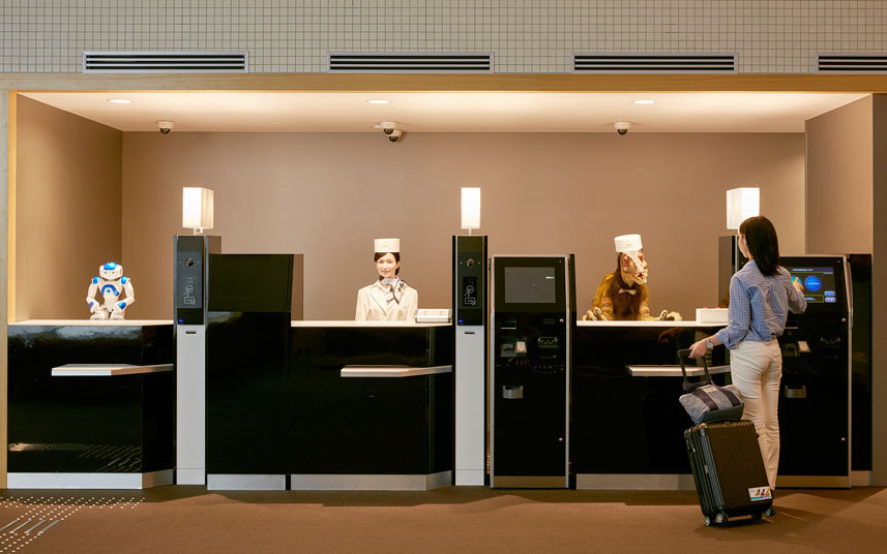
\includegraphics[width=0.75\linewidth]{images/roboter_rezeption_nagasaki.png}
\end{center}

\subsection{Der Mensch als „Bug“ des Systems}

Ein besonders wichtiges Beispiel
für die Ambivalenz menschlicher Fehlbarkeit
ist Stanislaw Petrow.

Petrow war Oberstleutnant
der sowjetischen Luftverteidigungsstreitkräfte.

Im Jahr 1983 meldete ein sowjetisches Frühwarnsystem
einen angeblichen Raketenangriff.

Petrow glaubte dem System jedoch nicht.

Seine Entscheidung verhinderte möglicherweise
eine militärische Katastrophe.

Dieses Beispiel zeigt,
dass menschliche Abweichung
nicht nur als Fehler verstanden werden kann.

Gerade weil Menschen zweifeln,
Kontext berücksichtigen
und technische Signale interpretieren können,
können sie in bestimmten Situationen
entscheidend sein.

Der Mensch ist also nicht einfach ein „Bug“ des Systems.

Er kann auch notwendig sein,
um Maschinenfehler zu erkennen
und technische Systeme kritisch zu überprüfen.

\subsection{Zur Geschichte der Künstlichen Intelligenz}

Die Geschichte der Künstlichen Intelligenz
weist einige historiographische Besonderheiten auf.

Sie lässt sich einerseits relativ schnell erzählen,
weil es vergleichsweise wenige grosse Entwicklungsschritte gibt.

Andererseits ist sie stark gegenwartsbezogen,
weil KI erst seit einigen Jahren
eine breite gesellschaftliche Relevanz besitzt.

Die Geschichte der KI lässt sich grob
in drei Phasen einteilen:

\begin{itemize}
\item Formalisierung von Denken und Denkprozessen
\item KI-Winter in den 1980er und 1990er Jahren
\item datengetriebene Modelle seit den 1980er Jahren mit Durchbruch in den 2010er Jahren
\end{itemize}

In der ersten Phase stand die Idee im Zentrum,
Denken so weit zu formalisieren,
dass es in Programmcode übersetzt werden kann.

Diese Idee kann je nach Perspektive
bis in die Antike,
in die Frühe Neuzeit
oder in die Mitte des 20. Jahrhunderts zurückverfolgt werden.

In der zweiten Phase,
dem sogenannten KI-Winter,
ging die Forschungsförderung zurück,
weil die Ergebnisse hinter den Erwartungen zurückblieben.

In der dritten Phase wurden Modelle
mit möglichst vielen Daten trainiert.

Diese datengetriebene Entwicklung
führte ab den 2010er Jahren
zu wichtigen Durchbrüchen.

\subsection{KI und die Frage nach Intelligenz}

Die Geschichte der KI ist eng verbunden
mit der Frage,
was Intelligenz eigentlich bedeutet.

Wer über KI nachdenkt,
denkt immer auch darüber nach,
was Menschen ausmacht.

Künstliche Intelligenz zwingt dazu,
menschliche Fähigkeiten zu definieren,
zu formalisieren
und mit maschinellen Leistungen zu vergleichen.

Dabei wird häufig spekuliert,
welche menschlichen Fähigkeiten
Maschinen übernehmen könnten.

Diese Spekulation betrifft nicht nur Rechnen
oder logisches Problemlösen,
sondern auch Sprache,
Wahrnehmung,
Entscheidung,
Kreativität
und soziale Interaktion.

Gerade deshalb ist KI nicht nur ein technisches,
sondern auch ein philosophisches,
soziales und politisches Thema.

\subsection{Schach als Leitmedium der KI-Forschung}

Ein wichtiges Beispiel in der Geschichte der KI
ist der Schachcomputer.

Schach wurde lange als Leitmedium
der KI-Forschung betrachtet.

Der Grund dafür liegt in der Struktur des Spiels.

Schach besitzt klare Regeln
und eine begrenzte Anzahl möglicher Züge,
auch wenn diese Anzahl sehr gross ist.

Damit eignet sich Schach gut,
um maschinelles Problemlösen zu testen.

Gleichzeitig zeigt das Beispiel aber auch
eine Einschränkung.

Schach bildet nur eine sehr enge Form von Intelligenz ab.

Es geht um logisches Problemlösen
in einem klar abgegrenzten Regelraum.

Andere Dimensionen menschlicher Intelligenz
spielen dabei keine Rolle.

Dazu gehören:

\begin{itemize}
\item Sprache
\item soziale Beziehungen
\item Widerspruch
\item Körperlichkeit
\item Emotion
\item Politik
\end{itemize}

Der Sieg von Deep Blue gegen Garri Kasparov 1997
wurde deshalb als Zeichen maschineller Überlegenheit verstanden.

Er zeigte aber vor allem,
dass Maschinen in klar definierten Aufgabenräumen
sehr leistungsfähig sein können.

\begin{center}
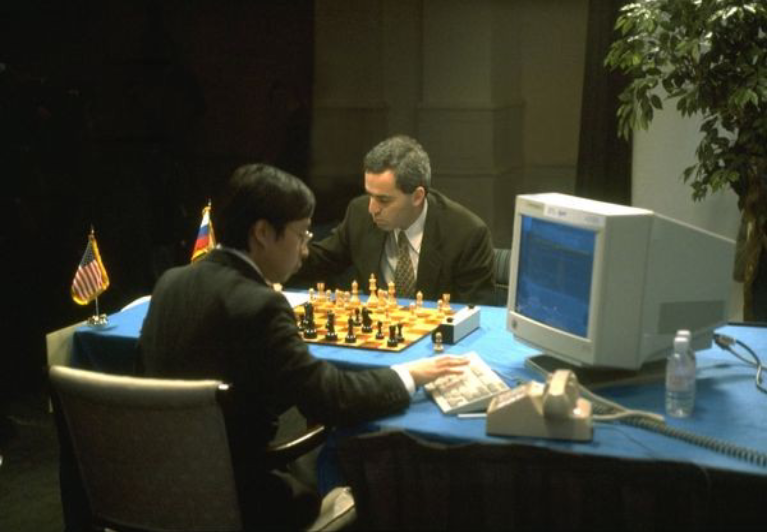
\includegraphics[width=0.75\linewidth]{images/kasparov_deep_blue.png}
\end{center}

\subsection{Fehlbarkeit von Mensch und Maschine}

Unter den Bedingungen des Schachs
erscheint der Mensch spätestens seit Deep Blue
auch im Bereich der Intelligenz unterlegen.

Wenn man jedoch Sprachmodelle wie ChatGPT betrachtet,
verschiebt sich diese Einschätzung.

Sprachmodelle arbeiten nicht in einem klar abgegrenzten Regelraum
wie dem Schachspiel.

Sie bewegen sich in offenen,
mehrdeutigen und sozialen Bedeutungsräumen.

Dadurch wird auch die Fehlerhaftigkeit der Maschine
wieder sichtbar.

Maschinen können falsche Informationen erzeugen,
Zusammenhänge missverstehen
oder scheinbar überzeugende Antworten geben,
die sachlich nicht stimmen.

Die Fehlbarkeit liegt daher nicht nur beim Menschen.

Auch Maschinen machen Fehler.

Entscheidend ist,
dass diese Fehler anders entstehen
und oft schwieriger zu erkennen sind.

\subsection{Digitale Technik und Wartung}

Von der Industrialisierung bis zur Mitte des 20. Jahrhunderts
wurden Maschinen häufig als Mittel verstanden,
um fehlbare Menschen zu entlasten,
zu unterstützen oder zu ersetzen.

Ab den 1960er Jahren,
besonders mit der Digitaltechnik,
veränderte sich dieses Verhältnis.

Der Mensch wurde zunehmend notwendig,
um komplexe Maschinen und Systeme
funktional am Laufen zu halten.

Fehlersuche,
Wartung,
Kontrolle und Anpassung
wurden zentrale Aufgaben.

Gleichzeitig wurden technische Systeme immer komplexer.

Menschen überblickten ihre Systeme
immer weniger vollständig.

Dadurch wurde die Fehlersuche
aufwändig,
ineffizient
und selbst wieder zu einem Problem,
das technisch gelöst werden sollte.

Technik erzeugt also nicht nur Entlastung,
sondern auch neue Arbeit.

\subsection{KI und die Neuordnung des Mensch-Maschinen-Verhältnisses}

Mit KI wird das Mensch-Maschinen-Verhältnis
noch einmal neu geordnet.

Die Frage lautet nicht mehr nur,
ob Maschinen Menschen ersetzen können.

Vielmehr geht es darum,
wer in komplexen Systemen
welche Rolle übernimmt.

KI-Systeme können menschliche Arbeit unterstützen,
aber auch menschliche Fehler reproduzieren.

Sie können Entscheidungen vorbereiten,
aber auch Verantwortung verschieben.

Wichtige Fragen sind daher:

\begin{itemize}
\item Wer kontrolliert KI-Systeme?
\item Wer erkennt Maschinenfehler?
\item Wer trägt Verantwortung für technische Entscheidungen?
\item Reproduziert KI menschliche Vorurteile?
\item Wann ist menschliches Eingreifen notwendig?
\end{itemize}

KI zeigt damit besonders deutlich,
dass die Grenze zwischen menschlicher
und maschineller Fehlbarkeit
nicht eindeutig ist.

Menschen machen Fehler.

Maschinen machen Fehler.

Und KI kann menschliche Fehler
in technische Systeme einschreiben,
verstärken und automatisieren.

\subsection{Zentrale Erkenntnisse}

Die Vorlesung zeigt,
dass die Geschichte der KI
nicht nur als Geschichte technischer Innovationen
verstanden werden kann.

Sie ist Teil einer längeren Technikgeschichte,
in der Menschen Maschinen entwickeln,
um Probleme zu lösen,
Arbeit zu erleichtern,
Effizienz zu steigern
und eigene Grenzen zu überwinden.

Zentrale Erkenntnisse sind:

\begin{itemize}
\item Technikentwicklung beruht auf verschiedenen Faktoren wie Problemlösung, Wachstum, Wissenschaft, Staat, Militär und sozialer Aushandlung.
\item Technik ist nicht neutral, sondern enthält gesellschaftliche Normen, Interessen und Menschenbilder.
\item Der Mensch wird in der Technikgeschichte häufig als fehlerhaftes Wesen beschrieben.
\item Maschinen erscheinen oft als überlegen, weil sie als rational, ausdauernd und neutral gelten.
\item Diese Vorstellung übersieht, dass auch Maschinen fehlerhaft sind.
\item KI verschiebt die Frage nach Fehlbarkeit, Verantwortung und Kontrolle neu.
\end{itemize}

Die zentrale These lautet:

KI verändert das Mensch-Maschinen-Verhältnis nicht,
weil Maschinen plötzlich vollkommen fehlerfrei wären.

Sie verändert es,
weil menschliche und maschinelle Fehlbarkeit
enger miteinander verbunden werden.

Die Geschichte der KI ist daher immer auch
eine Geschichte darüber,
wie Menschen sich selbst,
ihre Schwächen
und ihre Verantwortung
im Spiegel der Maschine verstehen.
